\chapter{System (or Project) Design and Architecture}
        % flowchart, description, Architecture

 

\section{Cycle-GAN}
\begin{figure}[htbp]
  \centering
  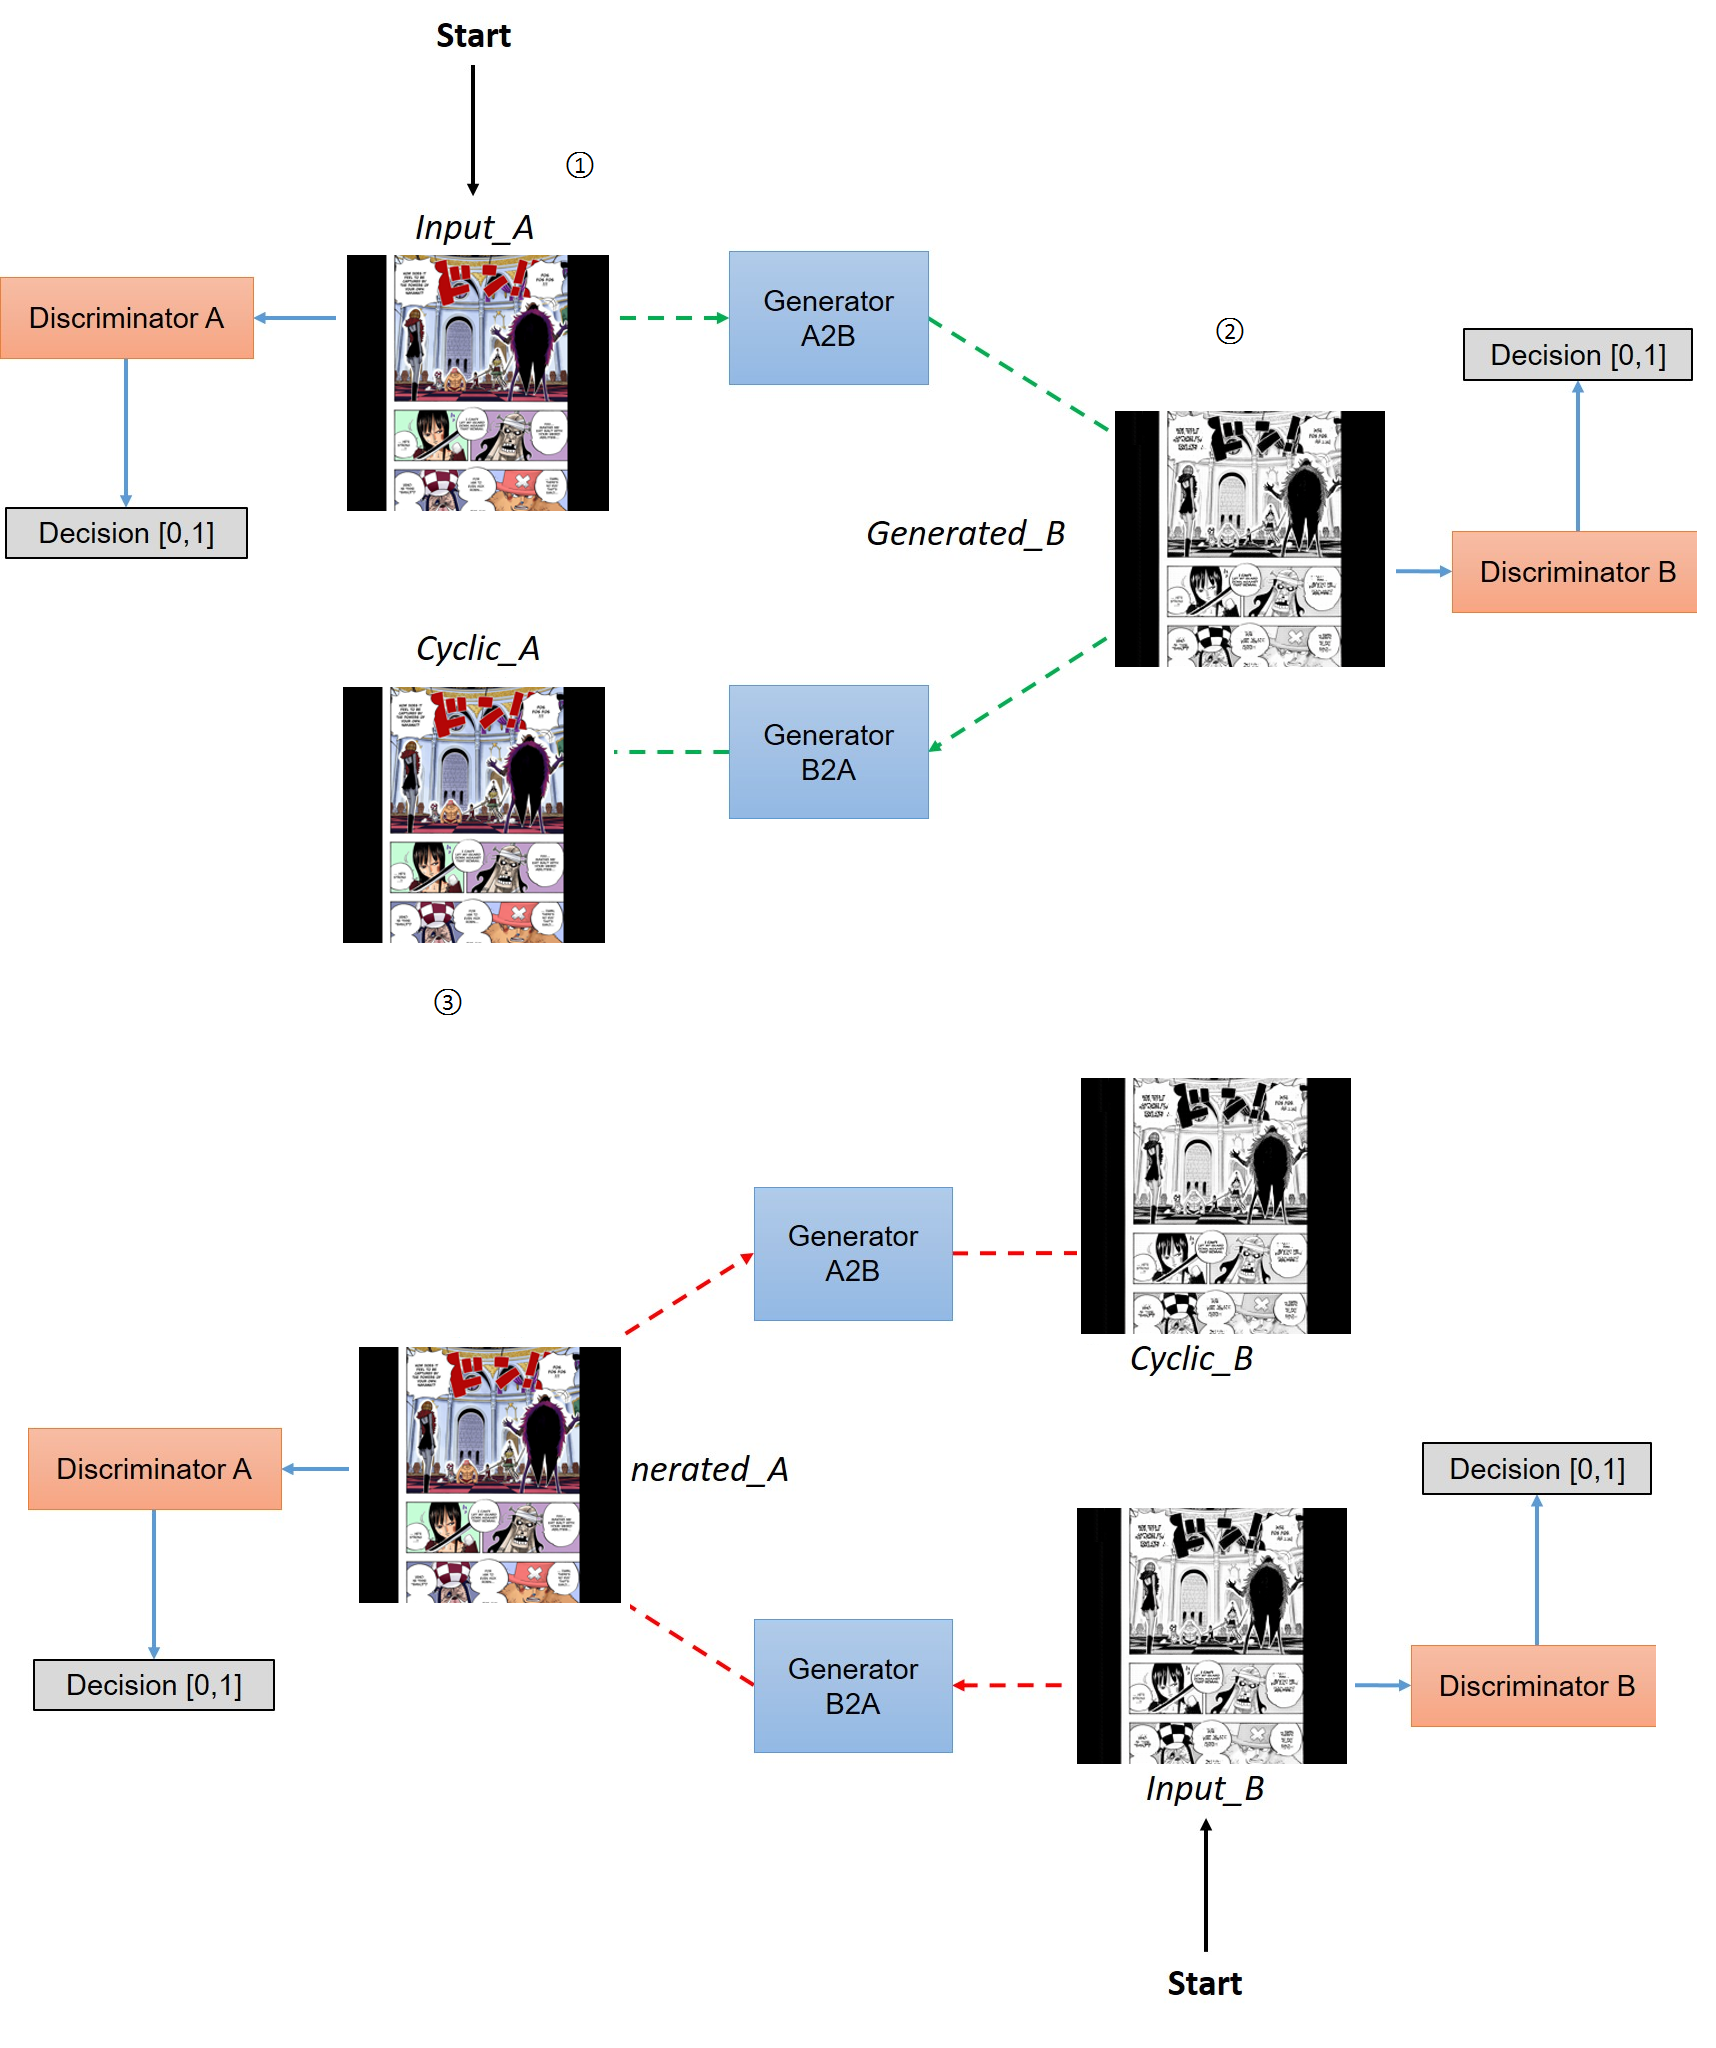
\includegraphics[width=0.8\textwidth]{img/GAN_block_diagram.png}
  \caption{Cycle-GAN implementation for manga colorization}
  \label{fig:cycle-gan-implementation}
\end{figure}
CycleGAN \cite{zhu2017unpaired} is a model proposed for performing image-to-image translations without paired data. The key idea behind CycleGAN is to learn mapping functions between two domains A and B such that the distribution of images from domain A mapped to domain B is similar to the distribution of images in domain B, and vice versa .
\pagebreak
CycleGAN consists of two GANs - G: A → B and F: Y → X. G tries to transform images from domain A to look like they came from domain B, and F does the opposite.

Along with the generators G and F, there are also two discriminators, DA and DB. DA tries to distinguish between images from domain A and generated images from F. Similarly, DB tries to distinguish between images from domain B and generated images from G. \cite{zhu2020unpaired}.
\\
       
\subsection{Generator}
The ResNet9 generator is a variant of the ResNet architecture adapted for use in generative adversarial networks (GANs) for image synthesis tasks. It employs deep residual blocks with skip connections to capture complex patterns in input noise, while normalization layers stabilize training. Activation functions introduce non-linearity, enabling the model to learn intricate mappings between noise and generated images.
The generator takes a black and white manga panel as input and learns to predict the corresponding colored version of the manga panel. The generator passes images through series of convolution layers with downsampling and upsampling to produce colored output. The generator architecture (figure \ref{fig:Generator Architecture}) is constructed as in \cite{simonyan2015deep}. 

\begin{figure}[h!]
  \centering
  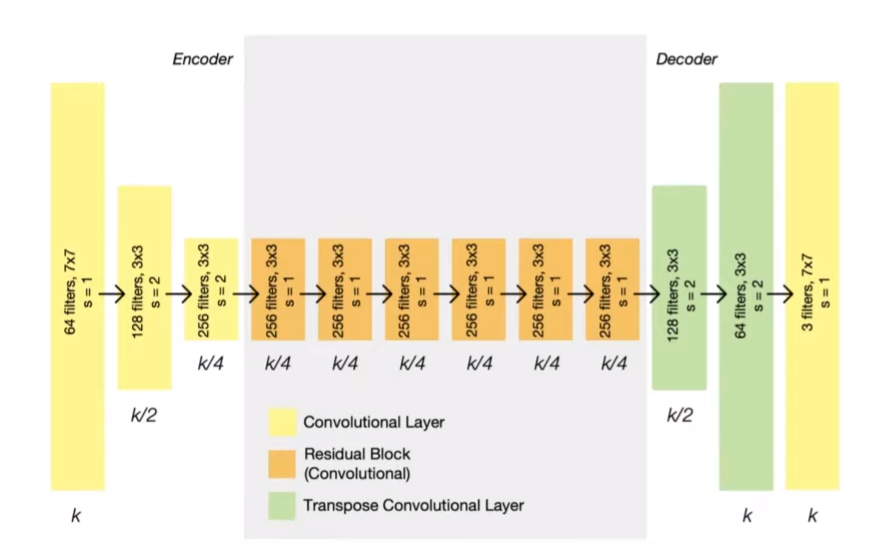
\includegraphics[width=0.8\textwidth]{img/generator (1).png}
  \caption{ResNet9 Generator Architecture }
  \label{fig:Generator Architecture}
\end{figure}

\subsection*{Input Processing}
The input image is initially processed through a series of layers to extract features. It starts with a reflection padding layer followed by a convolutional layer with a kernel size of 7 and 64 output channels.
Instance normalization is applied after the first convolutional layer, which normalizes the activations across the spatial dimensions of each channel independently for each sample in a batch.
\subsection*{Downsampling}
After the initial processing, the generator performs downsampling to reduce the spatial dimensions of the features while increasing the number of channels. This downsampling is achieved through two sets of convolutional layers with stride 2, effectively halving the spatial dimensions of the features while doubling the number of channels. Instance normalization and ReLU activation are applied after each downsampling operation.
\subsection*{Residual Blocks}
The core of the generator architecture consists of a series of residual blocks. These blocks aim to capture and refine image details across different scales. Each residual block contains two convolutional layers with 3x3 kernels, followed by instance normalization and ReLU activation. The input to each residual block is added to the output of the convolutional layers, allowing the network to learn residual mappings.
\subsection*{Upsampling}
After the residual blocks, the generator performs upsampling to reconstruct the high-resolution output image. Similar to the downsampling stage, upsampling is achieved through two sets of transposed convolutional layers. These layers increase the spatial dimensions while reducing the number of channels. Instance normalization and ReLU activation are applied after each upsampling operation.
\subsection*{Output Layer}
Finally, the upscaled features are passed through a reflection padding layer followed by a convolutional layer with a kernel size of 7 to generate the output image. The output image is normalized using the hyperbolic tangent (Tanh) activation function, which maps the pixel values to the range [-1, 1].

\begin{figure}[htbp]
    \centering
    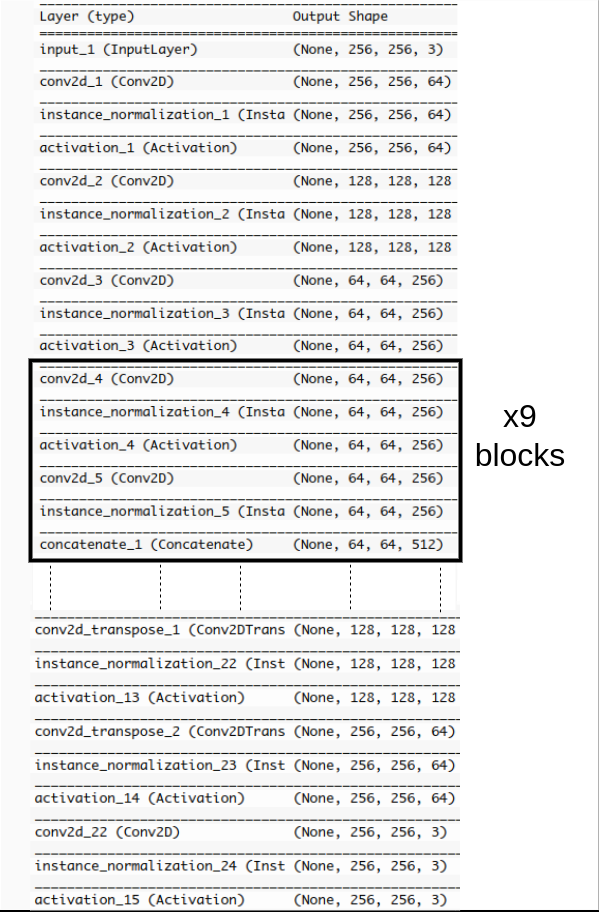
\includegraphics[width=0.8\textwidth]{chapter/output/gen_summary.png}
    \caption{Generator Architecture Summary}
    \label{fig:gen_summary}
\end{figure}

\pagebreak

\subsection{Discriminator}
The PatchGAN discriminator \cite{zhu2020unpaired} in CycleGAN is designed to discriminate between real and fake images at the patch level rather than the image level. It consists of convolutional layers with decreasing spatial dimensions and increasing channel depths.

\subsection*{Architecture}
The architecture follows a pattern of convolutional layers with increasing channel depths: C64-C128-C256-C512. Each layer is followed by a normalization step, often using instance normalization, and a non-linear activation function, typically Leaky ReLU.
\subsection*{Patch-Level Discrimination}
 Instead of outputting a single probability for the entire image, the discriminator outputs a matrix of probabilities corresponding to different patches of the input image. This patch-based approach allows the discriminator to capture fine-grained details and textures in both real and fake images.
 \subsection*{Final Layers}
 Although not mentioned in the paper \cite{zhu2020unpaired}, the discriminator includes a final hidden layer C512 with a stride of 1×1, followed by an output layer C1 also with a 1×1 stride, utilizing a linear activation function. This configuration enables the discriminator to produce an output feature map of size 16×16 when applied to an input image of size 256×256.
  \subsection*{Training Objective}
  The discriminator aims to minimize the classification error between real and fake patches, effectively learning to distinguish between authentic and generated image patches. \\
  
  By utilizing a PatchGAN discriminator, CycleGAN is able to enforce high-frequency structure consistency between input and output images, facilitating the translation of image style and domain adaptation tasks


%---------------------------------flowchart

\begin{figure}
  \centering
  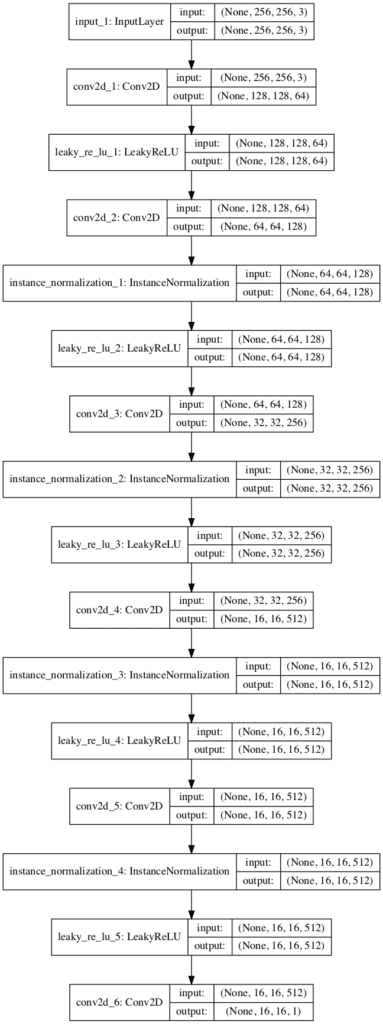
\includegraphics[height=1.25\textwidth]{img/discriminator_new.png}
  \caption{Discriminator Architecture }
  \label{Discriminator Architecture}
\end{figure}

\begin{figure}[p]
    \centering
    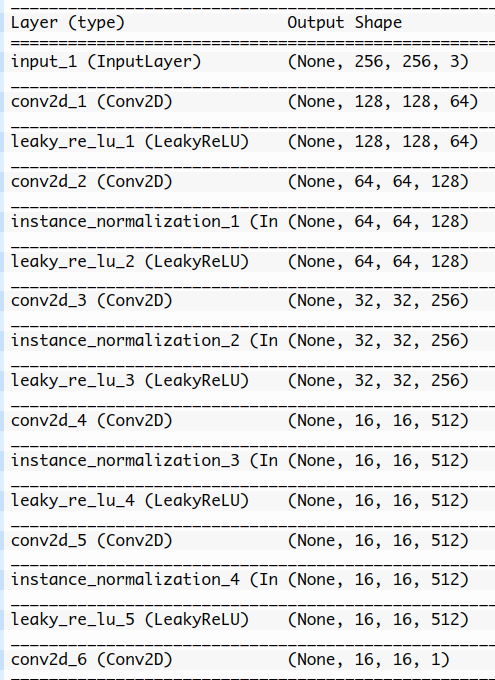
\includegraphics[width=1\textwidth]{chapter/output/disc_summary.png}
    \caption{Discriminator Architecture Summary}
    \label{fig:gen_summary}
\end{figure}




\newpage
\section{Loss Function}

To teach the model to generate similar colors for similar patterns and introduce a variety of colors, we use a mix of different loss functions.
\begin{itemize}
  \item \textbf{L1 Loss} \\
        In order to enforce the generator to produce similar coloring to the
        ground truth, we use a pixel level L1 metric that calculates the distance between
        output image $\mathcal{G}\left( x, d, h, \mathcal{E}\left( x \right)\right)$ and ground truth image y.
        \begin{equation}
          \mathcal{L}_{L_1}^\mathcal{G} = \|\mathcal{G}\left( x, d, h, \mathcal{E}\left( x \right)\right) - y \|
        \label{l1-loss}
        \end{equation}

        Where,
        \begin{itemize}
            \item $\mathcal{L}_{L_1}^\mathcal{G}$ = Generator L1 Loss
            \item $\mathcal{G}$ = Generator function
            \item x = Input to Generator
            \item d = Conditioning information
            \item h = Hidden state
            \item $\mathcal{E} (x)$ = Encoder function applied to input x
            \item y = Ground truth image
        \end{itemize}

  % \item \textbf{Perceptual Loss} \\
  %       To ensure similarity not only at the pixel level but also at the
  %       structural level, we use perceptual loss as described in \cite{10.1007/978-3-030-72610-2_17}. It’s an L2-loss based on
  %       the distance between some CNN feature maps for generated and ground truth
  %       images.

  %       \begin{equation}
  %         \mathcal{L}_{per}^\mathcal{G} = \frac{1}{chw}\| \mathcal{V} \left( \mathcal{G}\left( x, d, h, \mathcal{E}\left( x \right)\right)\right) - \mathcal{V}\left(y\right) \|
  %       \end{equation}
  %       Where, 
  %       \begin{itemize}
  %           \item $\mathcal{V}$ = a VGG-16 network
  %           \item c = number of channels
  %           \item h = height of feature maps
  %           \item w = width of feature maps
  %       \end{itemize}
      
  \item \textbf{Adversarial losses} \\
        For the mapping function G:X→Y and its discriminator D(y) , we express the objective as:
        \begin{equation}
          \mathcal{L}_\mathcal{G}{_{adv}}  =  \mathbb{E}_{x,h}[log\left( 1 - \mathcal{D} \left( \mathcal{G}_{main} \left( x, d \left( x \right), h, \mathcal{E} \left( x \right) \right) \right) \right)]
        \end{equation}
        where G tries to generate images G(x) that look similar to images from domain Y , while D(y) aims to distinguish between translated samples G(x) and real samples y. G aims to minimize this objective against an adversary D that tries to maximize it.

        We introduce a similar adversarial loss for the mapping
        function F : Y → X and its discriminator D(x) as well:
        \begin{equation}
          \mathcal{L}_D{_{adv}} = - \mathbb{E}_y [ log\mathcal{D}\left(y\right)] - \mathbb{E}_{x,h}[log\left(1 - \mathcal{D}\left(\mathcal{G}_{main}\left(x,d\left(x\right),h,\mathcal{E}\left(x\right)\right)\right)\right)]
        \end{equation}
        \pagebreak
  % \item \textbf{White Color Penalty Loss} \\
  %       We penalize the network if the pixel value is close to the maximum corresponding
  %       to the white color as found in \cite{10.1007/978-3-030-72610-2_17}. $\mathcal{L}_{white}$ is calculated as the mean square of the channel-wise
  %       sums (we assume that values of G output belong to [0, 1]).
  %       \begin{equation}
  %         \mathcal{L}_{white}^\mathcal{G} = \frac{\sum_{i,j,k}\left(white\_zones[i,j,k]\right)^2}{
  %           \sum_{i,j,k} mask[i,j,k] + 1
  %         }
  %       \end{equation}

  %       where,  $mask[i,j,k]$ is binary representation identifying the pixels in the color image exceeding a threshold of 0.85, and $white\_zones[i,j,k]$ represent the corresponding normalized bright regions in the genrated image.\\

  \item \textbf{Cycle Consistency Loss} \\
        Adversarial losses alone cannot guarantee that the learned function can map an individual input $x_i$ to a desired output $y_i$. To further reduce the space of possible mapping functions, the learned mapping functions should be cycle-consistent, for each image x from domain X, the image translation
        cycle should be able to bring x back to the original image,
        i.e., x → G(x) → F(G(x)) $\approx$ x. We encourage this behavior using a cycle consistency loss as found in \cite{zhu2020unpaired}:
        \begin{equation}
          \mathcal{L}_{cyc}\left(G,F\right) = \mathbb{E}_{x\sim p{_{data}}\left(x\right)}[\|F\left(G\left(x\right)\right) - x \|]
          + \mathbb{E}_{y\sim p{_{data}}\left(y\right)}[\|G\left(F\left(y\right)\right) - y\|]
        \end{equation}

        Where,
        \begin{itemize}
            \item $\mathcal{L}_{cyc}\left(G,F\right)$ = Cycle consistency loss between generators G and F
            \item $\mathbb{E}_{x\sim p{_{data}}\left(x\right)}$ = Expectation operator with respect to data distribution $p{_{data}}\left(x\right)$
            \item $\|.\|$ = Normalization operation
            \item $\mathbb{E}_{y\sim p{_{data}}\left(y\right)}$ = Expectation operator with respect to data distribution $p{_{data}}\left(y\right)$
            
        \end{itemize}

\end{itemize}

\section{Performance Evaluation Metrics}
Due to the architecture and domain similarity, we can use the same metrics as in \cite{huang2021fully} to evaluate the performance of our model.\\
\begin{itemize}
  \item \textbf{PSNR}: \\
       PSNR (Peak Signal-to-Noise Ratio) is a metric commonly used to measure the quality of reconstructed images or videos by comparing them to the original ones. It measures the ratio between the maximum possible power of a signal and the power of corrupting noise that affects the fidelity of its representation.

PSNR values are typically expressed in decibels (dB) and range from 0 to infinity. Higher PSNR values indicate higher image quality, with values closer to infinity representing perfect reconstruction.

In practical terms, PSNR values above 30 dB are often considered excellent, while values below 20 dB may indicate significant loss of quality.:
        \begin{equation}
          PSNR = 10 * log_{10}\left(\frac{MAX_I^2}{MSE}\right)l
        \end{equation}
        where, MAX  is the maximum possible pixel value of the image, (like 255 for 8-bit image). Mean Square Error (MSE) is an objective criterion between predicted images and real images, which is represents as:
        \begin{equation}
          MSE = \frac{1}{mn} \sum_{i=0}^{m-1} \sum_{j=0}^{n-1} \|T(i, j) - F(i, j)\|^2 l
        \end{equation}
        m , n represent the size of the real image and the colorized image respectively.\\

  \item \textbf{SSIM}:\\
        SSIM (Structural Similarity Index Measure) is a metric used to quantify the similarity between two images. It takes into account three components: luminance, contrast, and structure, to evaluate how closely the images resemble each other perceptually.

The SSIM values range from -1 to 1, where 1 indicates perfect similarity between the images, 0 indicates no similarity, and -1 indicates perfect dissimilarity. Typically, values above 0.9 are considered excellent, indicating high similarity between the images.
        \begin{equation}
          SSIM = \frac{(2\mu_x\mu_y + c_1)(\sigma_{xy} + c_2)}{(\mu_x^2 + \mu_y^2 + c_1)(\sigma_x^2 + \sigma_y^2 + c_2)}
        \end{equation}

        \begin{equation}
          c_1 = (k_1 L)^2 \quad c_2 = (k_2 L)^2
        \end{equation}
        where
        \begin{itemize}
          \item \( \mu_x \) is the mean of image x,
          \item \( \mu_y \) is the mean of image y,
          \item \( \sigma_x^2 \) is the variance of image x,
          \item \( \sigma_y^2 \) is the variance of image y,
          \item \( 	\sigma_{xy} 	\) is the covariance of image x and image y,
          \item L is dynamic range of pixel values, usually L is equal to 255,
          \item \( k_1 = 0.01\) and \( k_2 = 0.03\) which are constants for stability.
        \end{itemize}

\end{itemize}